%&pdflatex
\documentclass{article}
\usepackage[final]{nips_2017}
\usepackage[utf8]{inputenc} % allow utf-8 input
\usepackage[T1]{fontenc}    % use 8-bit T1 fonts
\usepackage{hyperref}       % hyperlinks
\usepackage{url}            % simple URL typesetting
\usepackage{booktabs}       % professional-quality tables
\usepackage{amsfonts}       % blackboard math symbols
\usepackage{nicefrac}       % compact symbols for 1/2, etc.
\usepackage{microtype}      % microtypography
\usepackage{amsmath}
\usepackage{mathtools}
\usepackage{graphicx}
\usepackage{morefloats}
\usepackage{float}
\usepackage{listings}
\usepackage[usenames,dvipsnames]{xcolor}
\usepackage{commath}
\usepackage{graphicx}

% Define the coloring for keywords in Julia
\lstdefinelanguage{Julia}%
{morekeywords={abstract,break,case,catch,const,continue,do,else,elseif,%
    end,export,false,for,function,immutable,import,importall,if,in,%
    macro,module,otherwise,quote,return,switch,true,try,type,typealias,%
    using,while},%
  sensitive=true,%
  morecomment=[l]\#,%
  morecomment=[n]{\#=}{=\#},%
  morestring=[s]{"}{"},%
  morestring=[m]{'}{'},%
}[keywords,comments,strings]%

% Set the lstlistings to the Julia color scheme
\lstset{
  basicstyle       = \ttfamily,
  columns          = fullflexible,
  frame            = single,
  breaklines       = true,
  language         = Julia,
  basicstyle       = \ttfamily,
  keywordstyle     = \bfseries\color{blue},
  stringstyle      = \color{magenta},
  commentstyle     = \color{ForestGreen},
  showstringspaces = false,
  numbers          = left,
  xleftmargin      = 2em,
  framexleftmargin = 2em
}

\title{Scale Space Edge Detection}

\author{
  Nick Draper, Jonathan Hayase\\
  Seminar in Differential Geometry\\
  Harvey Mudd College
}

\begin{document}
\maketitle

\begin{abstract}
  Scale space representation is the idea that a two dimensional image can be represented by a collection of smoothed images.
  This paper documents how using such a representation can be useful for detecting edges in an image.
  The scale space allows for a classification of how strong different edges are in the image from very fine to coarse ones. 
\end{abstract}

\section{Edge Detection Background}
Detecting edges in images has long been a problem with many uniques solutions to approach it.
Generally speaking, the majority of algorithms are usually checking the image for some of the following features:

\begin{itemize}
\item large discontinuities in luminance values
\item discontinuities in different object orientations
\item large discontinuities in the intensity gradient
\end{itemize}

\indent Some of the common methods for edge detection include the Sobel, Canny, Prewitt, Roberts, and Fuzzy Logic algorithms.
However, these methods do not yield a lot of imformation with regards to the strength of the edges detected.
The majority of these algorithms will usually convolve the image with a static matrix to caclulate edges and does adapt enough to the image. 

This is why for our edge detection method, we will be using the scale space approach.
The benefit of using a scale space appraoch for edge detection, is we have the ability to classify the strength of the edges in the image.
This allows for a range of edges from very large immediate changes in intensity to very gradual.

\section{Scale Space and Its Derivatives}
To understand how exactly we detect images in the scale space, we must first define what the scale space is.
If we have a continuous function of multiple variables such as $f(x,y)$, then we define the scale space representation of such a function as 

\begin{equation}
  L(x;t) = g(x,y;t) * f(x,y)
\end{equation}

Here $t$ represents the scale parameter, and can be thought of how much smoothing is applied to the function. The function $g$ is the Gaussian kernel given by

\begin{equation}
  g(x,y;t) = \frac{1}{2 \pi t}e^{-(x^2+y^2)/(2t)}
\end{equation}

With the scale space representation defined, we can now take derivatives of it as it is a continuous well-defined function.
Spatial derivatives are relatively simple being defined as the following

\begin{equation}
  L_{x^{\alpha}y^{\beta}}(\cdot;t) = \partial_{x^{\alpha}y^{\beta}}L(\cdot;t) = g_{x^{\alpha}y^{\beta}}(\cdot;t) * f(\cdot)
\end{equation}

However, when taking the partial derivative with respect to the scale $t$, it becomes more interesting.
The scale space representation collection is a solution for the diffusion equation. Therefore is has the useful property of 

\begin{equation}
  \partial_t L = \frac{1}{2} \nabla^2 L = \frac{1}{2} (\partial_{xx} + \partial_{yy})L
\end{equation}

with the inital condition of $L(x,y;0) = f(x,y)$.
So now, scale derivatives can be represented as spatial derivatives. 

Now all these representations and operators are useful for continuous functions, but the images we deal with are discrete and contain quantized inetsnity values.
So we must now understand how these operations and properties apply to the discrete domain.

The scale space representation is still defined in a similar fashion.
The following is the discrete version of the scale space operationg on the function $f(x)$, which only has a single spatial variable.

\begin{equation}
  L(x;t) = (T(\cdot;t) * f(\cdot))(x;t)
\end{equation}

In this expression, $T$ represents the discrete version of the Gaussian kernel and is further evaluated as

\begin{equation}
  T(n;t) = e^{-t}I_n(t)
\end{equation}

where $I_n$ is the modified Bessel functions of integer order given by

\begin{equation}
  I_n(x) = i^{-\alpha}J_{\alpha}(ix) = \sum_{m=0}^{\infty}\frac{1}{m!\Gamma(m+\alpha+1)}\left(\frac{x}{2}\right)^{2m+\alpha}
\end{equation}

Now that the one dimensional case is understood for the scale space, we can expand this to two dimensions.
After all, images are compsed of two dimesnisons, so it makes sense that these operators can act on two dimensional functions.
The two dimensional scale space representation for discrete variables is given by the following

\begin{equation}
  L(x,y;t) = \sum_{m=-\infty}^{\infty}\sum_{n=-\infty}^{\infty}T(m;t)T(n;t)f(x-m,y-n)
\end{equation}

Even with the discrete case, the scale space representation must still satisfy the semidiscretized version of the diffusion equation.
Therefore by taking a scale derivative of the function we must have the following

\begin{equation}
  \partial_t L = \frac{1}{2}((1-\gamma)\nabla^2_5L+\gamma\nabla^2_\times L)
\end{equation}

where $\gamma \in [0,1]$ is a hyperparameter and,

\begin{equation}
  (\nabla^2_5f)_{0,0} = f_{-1,0} + f_{+1,0} + f_{0,-1} + f_{0,+1} - 4f_{0,0}
\end{equation}
\begin{equation}
  (\nabla^2_\times f)_{0,0} = \frac{1}{2}(f_{-1,-1} + f_{-1,+1} + f_{+1,-1} + f_{+1,+1} - 4f_{0,0})
\end{equation}

Note that $f_{-1,1}$ represents $f(x-1, y+1)$. Now that we have defined what discrete scale spaces and their derivatives look like, we can start to define what an edge is.

\section{Defining an Edge in Scale Space}
We classify edge points as points which have gradient magnitueds that assume a maximum in the direction of the gradient. Let us denote the magnitude of the gradient of $L$ as $L_g$. Then we define an edge in the scale space with the following conditions

\begin{equation} \label{eq:c1}
  \begin{aligned}
    L_{gg} &= 0 \\
    L_{ggg} &< 0
  \end{aligned}
\end{equation}

The way we can then represent these conditions in terms of spatial derivatives is as follows

\begin{equation}
  \begin{aligned}
    L_{gg} &= L_x^2L_{xx}+2L_xL_yL_{xy}+L_y^2L_{yy} = 0 \\
    L_{ggg} &= L_x^3L_{xxx} +3L_x^2L_yL_{xxy}+3L_xL_y^2L_{xyy}+L_y^3L_{yyy} < 0
  \end{aligned}
\end{equation}

This is useful for determining edges at a single scale, but if we are to determine edges over multiple scales, we must also develop an edge strength metric, $\varepsilon_{norm}L$.
Thus this adds two more conditions that must be satisified for an edge to be classified in the scale space. 

\begin{equation} \label{eq:c2}
  \begin{aligned}
    \partial_t(\varepsilon_{norm}L(x,y;t)) = 0\\
    \partial_{tt}(\varepsilon_{norm}L(x,y;t)) < 0
  \end{aligned}
\end{equation}

Then equation \ref{eq:c1} in conjunction with \ref{eq:c2} form the neccessary constraints for us to define an edge in the scale space.
Now we must define what we mean by edge strength and give a clearer idea of $\varepsilon_{norm}$.

The approach we took was to let our edge strength meteric be defined by the gradient magnitude that has been normalized by our $\gamma$ factor.
In this case we can define it as 

\begin{equation}
  \begin{aligned}
    G_{\gamma}L &= L_{g,\gamma}^2 \\
    &= t^{\gamma}(L_x^2+L_y^2)
  \end{aligned}
\end{equation}

Then the strength of the edges is found by computing the path integral over the maximal connected edge $\Gamma$ given by

\begin{equation}
  G(\Gamma) = \int_{(x;t) \in \Gamma} \sqrt{(G_{\gamma}L)(x;t)} \,\, \dif s
\end{equation}

where $\dif s^2=\dif x^2+\dif y^2$.

\section{Implementation}
For our implementation we will be using the following image to run our tests on

\begin{figure}[H]
  \centering
  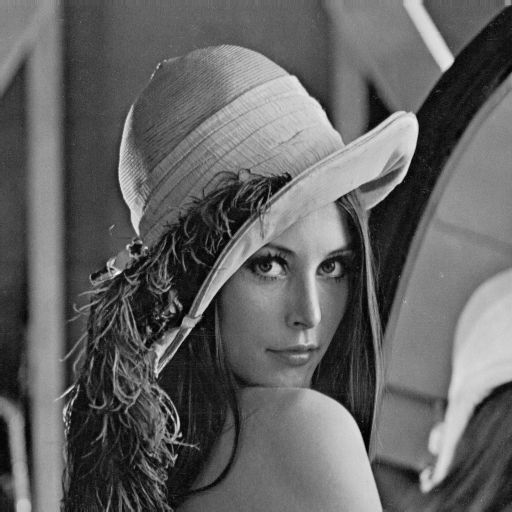
\includegraphics[scale=0.5]{Images/lena.jpg}
  \caption{Original Grayscale Lena Image}
  \label{lena_o}
\end{figure}

Figure \ref{lena_o} is a standard test image for image processing and is good for our purposes since it contains a variety of different edges with different strengths.

So what we first do is define our convolution functions that we will be using in code.

\begin{lstlisting}
function combine_kernels(kers...)
    return reduce(conv2, kers)
end

function convolve_image(I, kers...)
    kernel = combine_kernels(kers...)
    return imfilter(I, centered(kernel))
end

function convolve_scale_space(L, kers...)
    return mapslices(
        scale_slice -> convolve_image(scale_slice, kers...),
        L,
        (1,2)
    )
end

function convolve_gaussian(img, sigma)
    # The dimension of the convolution matrix
    length = 8*ceil(Int, sigma) + 1
    return imfilter(img, reflect(Kernel.gaussian((sigma, sigma), (length, length))))
end
\end{lstlisting}

These will be used for computing all the neccessary two dimensional matrix convolutions that we will use throughout the rest of the code.
The next step is to then define our range of scales used and which derivative kernels we will be using to compute two dimensional discrete spatial derivatives.
The following code shows the definitions for our variables that will be used for all further calculations. 

\begin{lstlisting}
# Parameters
gamma = 1
scales = exp.(linspace(0, log(50), 40))

# Load the image
img = float.(ColorTypes.Gray.(testimage("lena_color_512")))

# Define derivative convolution matrices
Dy = Array(parent(Kernel.ando5()[1]))
Dx = Array(parent(Kernel.ando5()[2]))

# Normalized the derivatives
Dx /= sum(Dx .* (Dx .> 0))
Dy /= sum(Dy .* (Dy .> 0))
\end{lstlisting}

The derivative matrices used for our project are the ando5 matrices which are defined as the following

\begin{equation}
  \begin{aligned}
    [D_y] &=
    \begin{bmatrix}
      -0.003776 &-0.010199  &0.0  &0.010199  &0.003776 \\
      -0.026786 &-0.070844  &0.0  &0.070844  &0.026786 \\
      -0.046548 &-0.122572  &0.0  &0.122572  &0.046548 \\
      -0.026786 &-0.070844  &0.0  &0.070844  &0.026786 \\
      -0.003776 &-0.010199  &0.0  &0.010199  &0.003776
    \end{bmatrix} \\
    [D_x] &= [D_y]^T
  \end{aligned}
\end{equation}

From this point, we then can compute the scale space representation of our image and compute its spatial derivatives
The following section of code defines just how to do that.

\begin{lstlisting}
# Scale space representation
L = cat(3, (convolve_gaussian(img, sigma) for sigma in scales)...)

# First order derivatives
Lx = convolve_scale_space(L, Dx)
Ly = convolve_scale_space(L, Dy)

# Second order derivatives
Lxx = convolve_scale_space(Lx, Dx)
Lxy = convolve_scale_space(Lx, Dy)
Lyy = convolve_scale_space(Ly, Dy)

# Third order derivatives
Lxxx = convolve_scale_space(Lxx, Dx)
Lxxy = convolve_scale_space(Lxx, Dy)
Lxyy = convolve_scale_space(Lxy, Dy)
Lyyy = convolve_scale_space(Lyy, Dy)
\end{lstlisting}

By convolving our ando5 derivative matrix with the scale space representation, we can take spatial derivatives in both the $x$ and $y$ dimension. To give an idea of what the images look like, we have the following spatial derivatives of the image below.

\begin{figure}[H]
  \centering
  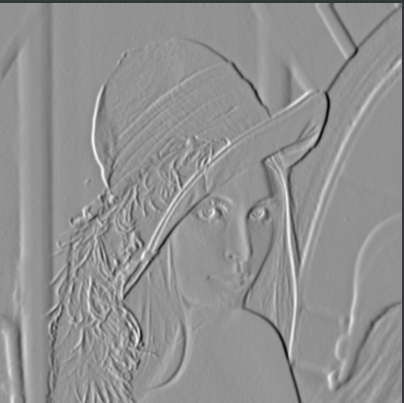
\includegraphics[scale=0.5]{Images/lx.png}
  \caption{Derivative of image in $x$ direction}
  \label{lx}
\end{figure}

\begin{figure}[H]
  \centering
  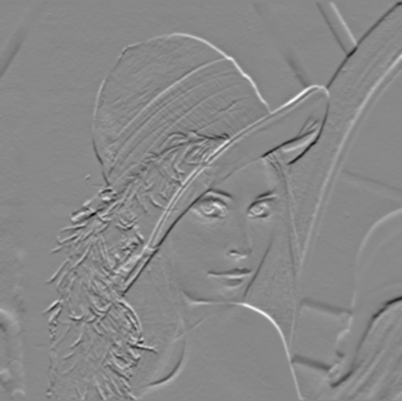
\includegraphics[scale=0.5]{Images/ly.png}
  \caption{Derivative of image in $y$ direction}
  \label{ly}
\end{figure}

Now that we have computed the spatial derivatives of the scale space representation of the image, we can check if we fulfill the conditions in (\ref{eq:c1}). 
The next step is to then calculate the edge strength derivatives neccessary to fulfill the conditions of (\ref{eq:c2}).
The code block below shows the computations for the edge strength based on the gradient magnitude and its derivatives.

\newpage

\begin{lstlisting}
# Shape the scales vector to be a vector with depth
scales3 = reshape(scales, 1, 1, length(scales))

# Definition of the gradient edge strength (magnitude)
const GL = scales3.^(gamma).*(Lx.^2+Ly.^2)

# Derivative of edge strength gradinet with respect to scale
const GLt = @. gamma*scales3^(gamma-1)*(Lx^2 + Ly^2) + scales3^gamma*(Lx*(Lxxx + Lxyy) + Ly*(Lxxy + Lyyy))

# Second derivative of edge strength gradinet with respect to scale
const GLtt = @. (gamma*(gamma - 1)*scales3^(gamma - 2)*(Lx^2 + Ly^2) + 2gamma*scales3^(gamma-1)*(Lx*(Lxxx + Lxyy) + Ly*(Lxxy + Lyyy)) + scales3^gamma/2*((Lxxx + Lxyy)^2 + (Lxxy + Lyyy)^2 + Lx*(Lxxxxx + 2Lxxxyy + Lxyyyy) + Ly*(Lxxxxy + 2Lxxyyy + Lyyyyy))) < 0
\end{lstlisting}



\section*{Appendix}

\lstinputlisting[caption={edge\_detect.jl},label=edge_detect,frame=none]{edge_detect.jl}

\section*{References}

\end{document}
